\chapter{Cell structure}\label{cell-structure}

The smallest unit of life is the
\href{https://en.wikipedia.org/wiki/Cell_(biology)}{cell}. In this lab,
we will look at eukaryotic (plant and animal) cells under the
microscope.

\begin{figure}

{\centering 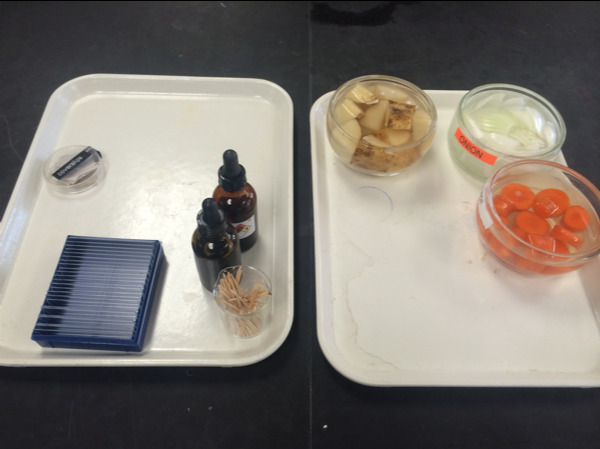
\includegraphics[width=0.7\linewidth]{./figures/cell_struc/materials}

}

\caption{Experimemntal materials}\label{fig:materials}
\end{figure}

\section{Elodea cells}\label{elodea-cells}

\subsection{Experimental procedures}\label{experimental-procedures-7}

\begin{enumerate}
\def\labelenumi{\arabic{enumi}.}
\tightlist
\item
  Get a single leaf from the Elodea plant and mount it on a slide, cover
  it with a drop of water and a cover slip.
\item
  Look at the leaf under the microscope (Figure \ref{fig:elodea}).
\item
  Notice that the cells are clearly delineated by the cell wall. Inside
  the cells are large oval-shaped green bodies, the chloroplasts.
\end{enumerate}

\begin{figure}

{\centering 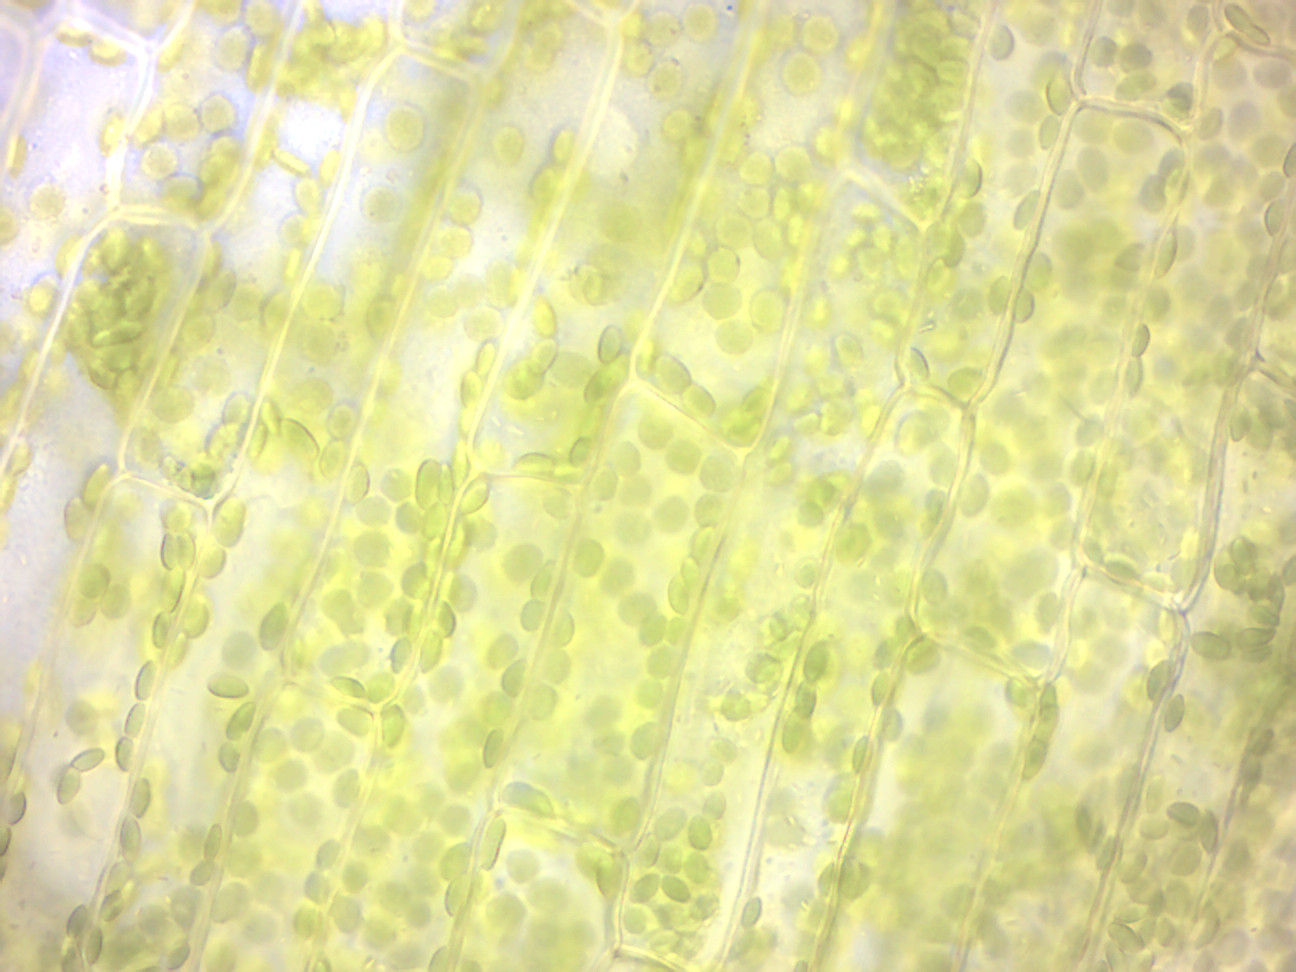
\includegraphics[width=0.7\linewidth]{./figures/cell_struc/elodea} 

}

\caption{Elodea wet mount (100× oil immersion objective).}\label{fig:elodea}
\end{figure}

\section{Onion leaf epidermal cells}\label{onion-leaf-epidermal-cells}

\subsection{Experimental procedures}\label{experimental-procedures-8}

\begin{enumerate}
\def\labelenumi{\arabic{enumi}.}
\tightlist
\item
        Peel a thin layer of cells from the concave side of a piece of onion as shown in Figure \ref{fig:onionpeel}.
\item
  Put the onion layer onto a new slide. Make sure the onion lays very flat and is not wrinkled or folded on your slide.
\item
  You may use a razor blade and cut both sides of the onion so that you are left with a small rectangular piece of onion in the center of your slide.
\item
  Add a drop of water on top of the small piece of onion in the center of your slide.
\item
  Add a coverslip on top.
\item
  Dim the light and find the nucleus, which is much easier to see here
  because there are no chloroplasts (Figure \ref{fig:onion}). Close examination should reveal one
  or more nucleoli in the nucleus.
\item
  Note the movement of small particles in the nearly trans- parent
  cytoplasm. This is Brownian movement, which we will study in more
  detail in another exercise.
\end{enumerate}

\begin{figure}

{\centering \includegraphics[width=0.7\linewidth]{./figures/cell_struc/onionpeel} 

}

\caption{Peel a thin layer of cells off the convave side of an onion slice.}\label{fig:onionpeel}
\end{figure}


\begin{figure}

{\centering 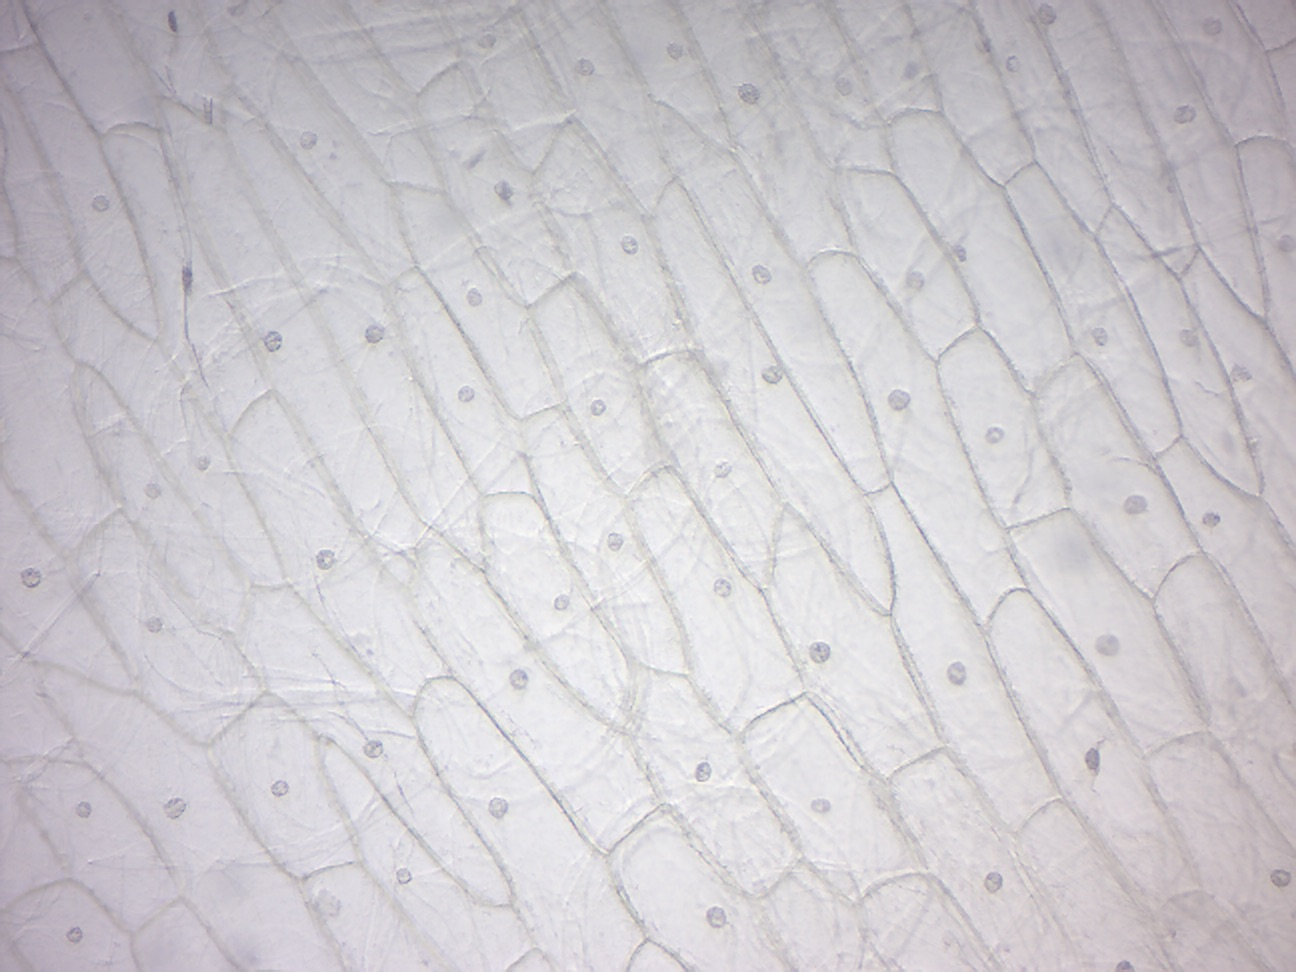
\includegraphics[width=0.7\linewidth]{./figures/cell_struc/onion} 

}

\caption{Onion epidermis.}\label{fig:onion}
\end{figure}


\section{Carrot root cells}\label{carrot-root-cells}

\subsection{Experimental procedures}\label{experimental-procedures-9}

\begin{enumerate}
\def\labelenumi{\arabic{enumi}.}
\tightlist
\item
  Use a razor blade and shave a very thin (almost translucent) slice of
  carrot onto a slide and prepare a wet mount of it (Figure \ref{fig:carot}).
\item
  Observe the orange-yellow bodies called chromoplasts, another type of
  plastid. Chromoplasts are enriched in pigments that give flowers,
  fruits, and fall leaves their colors, and carrots their orange color.
\end{enumerate}

\begin{figure}

{\centering 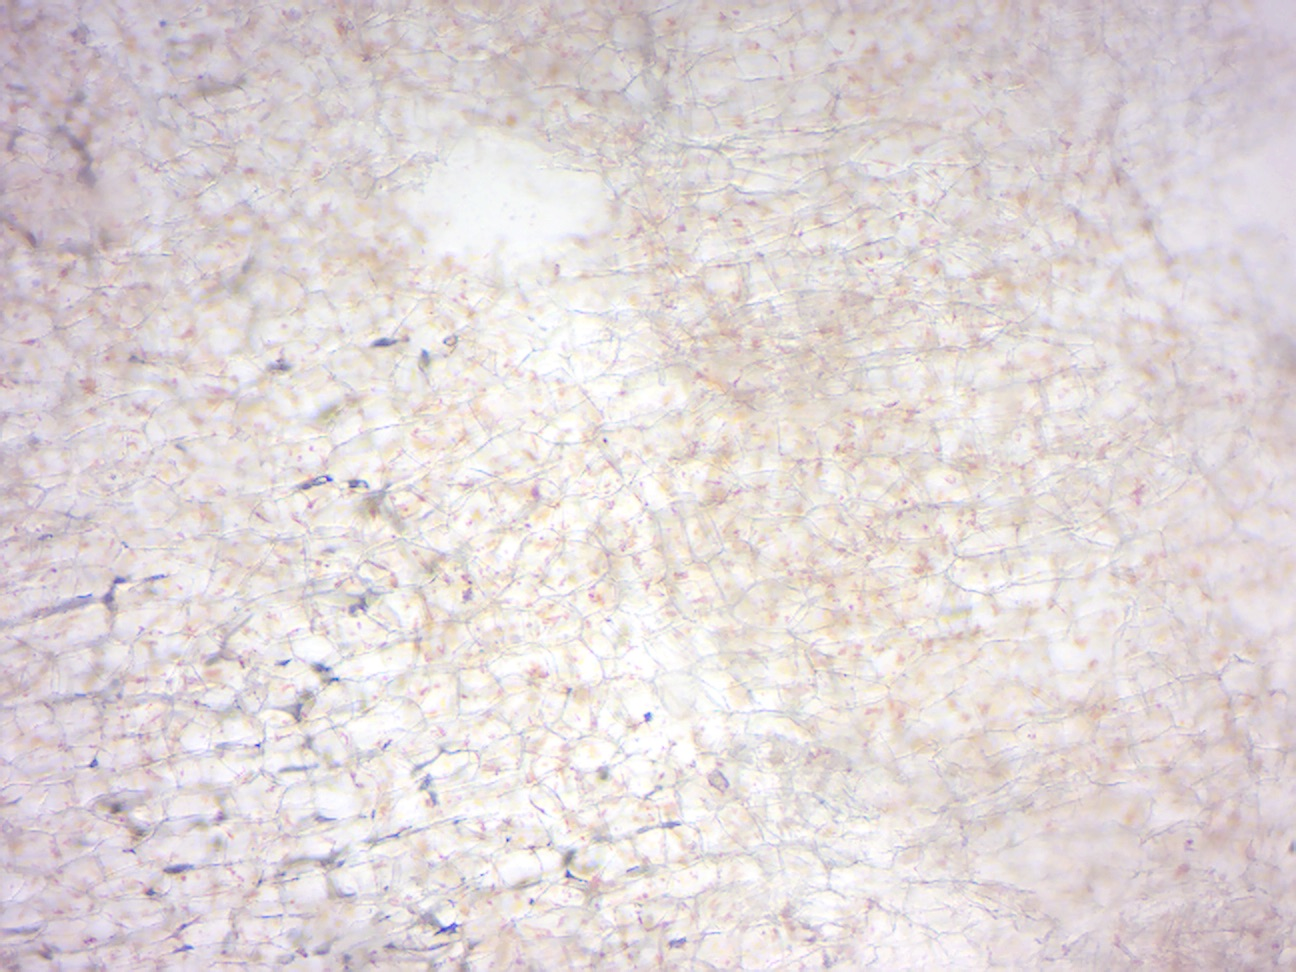
\includegraphics[width=0.7\linewidth]{./figures/cell_struc/carot} 

}

\caption{Carrot wet mount.}\label{fig:carot}
\end{figure}

\section{Potato cells}\label{potato-cells}

Potatoes are stems full of starch that is stored within the cells in
colorless plastids called amyloplasts (Figure \ref{fig:potato}).

\subsection{Experimental procedures}\label{experimental-procedures-10}

\begin{enumerate}
\def\labelenumi{\arabic{enumi}.}
\tightlist
\item
  Cut a very thin wedge-shaped sliver of potato.
\item
  Place it on a microscope slide.
\item
  Add a drop of iodine on top of the slice of potato.
\item
  Place a coverslip on top.
\item
  Observe the potato slice under the microscope.
\item
  Iodine stains starch a purple or blue-black color.
\end{enumerate}

\begin{figure}

{\centering 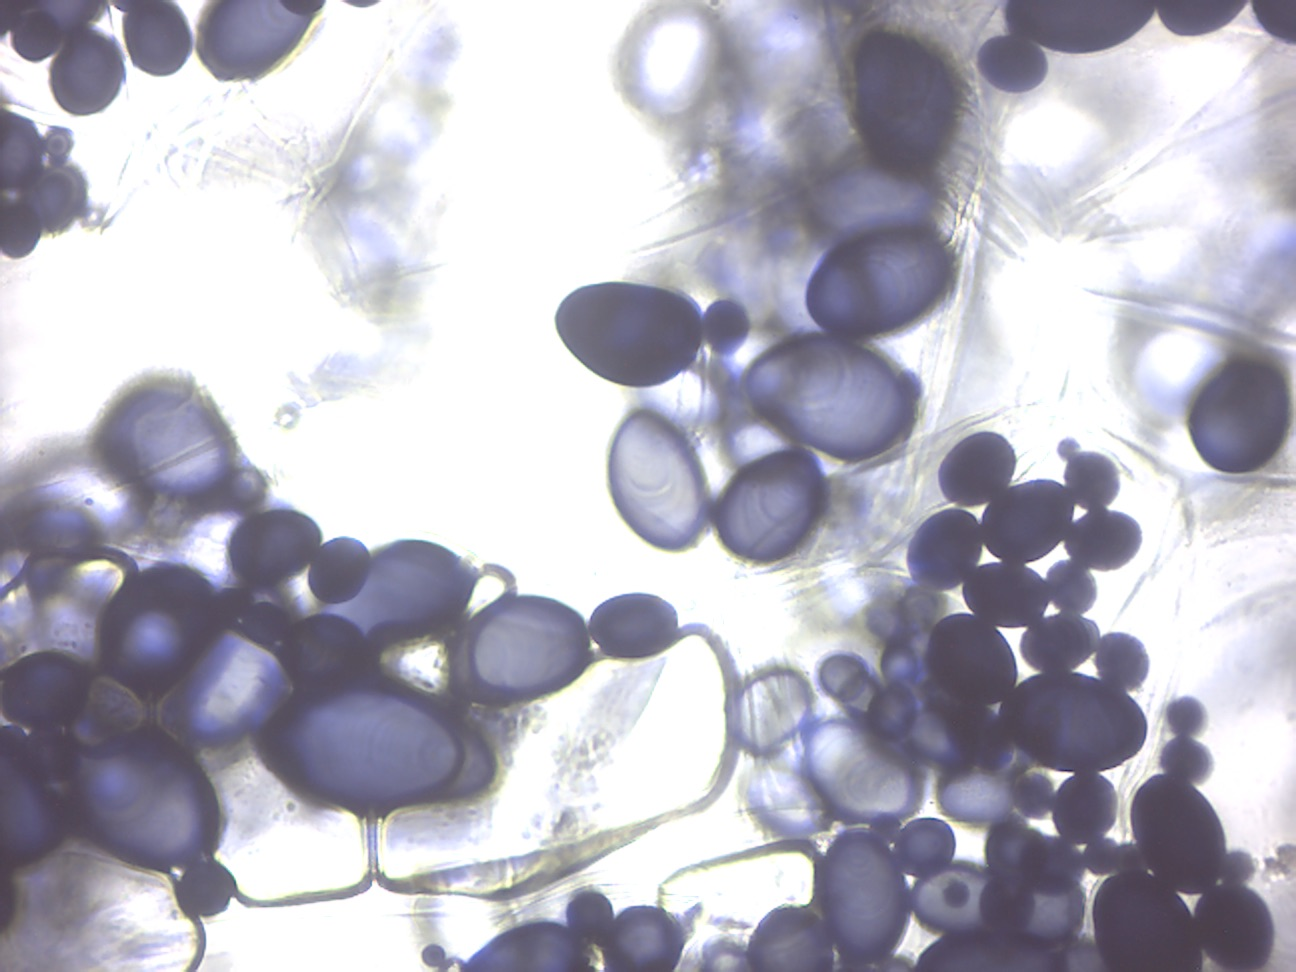
\includegraphics[width=0.7\linewidth]{./figures/cell_struc/potato} 

}

\caption{Amyloblasts in potato cells. The starch inside of the amyloplasts is stained blue-black by the iodine solution.}\label{fig:potato}
\end{figure}


\section{Cleaning up}\label{cleaning-up-3}

Discard the used glass slides in the container marked ``Broken glass''
in the fume hood.

\section{Human cheek cells}\label{human-cheek-cells}

The outer and inner surface of our body is formed by epithelial cells.

\subsection{Experimental procedures}\label{experimental-procedures-11}

\begin{enumerate}
\def\labelenumi{\arabic{enumi}.}
\tightlist
\item
  Rub the inner side of your cheek with a toothpick to pick up some
  cells.
\item
  Scrape the cloudy (cell-containing) fluid onto a slide, add a drop of
  dilute methylene blue, and observe under the microscope (Figure \ref{fig:cheek}). Note that
  bacteria and possibly fungi on top and around your cheek cells.
\end{enumerate}

\begin{figure}

{\centering 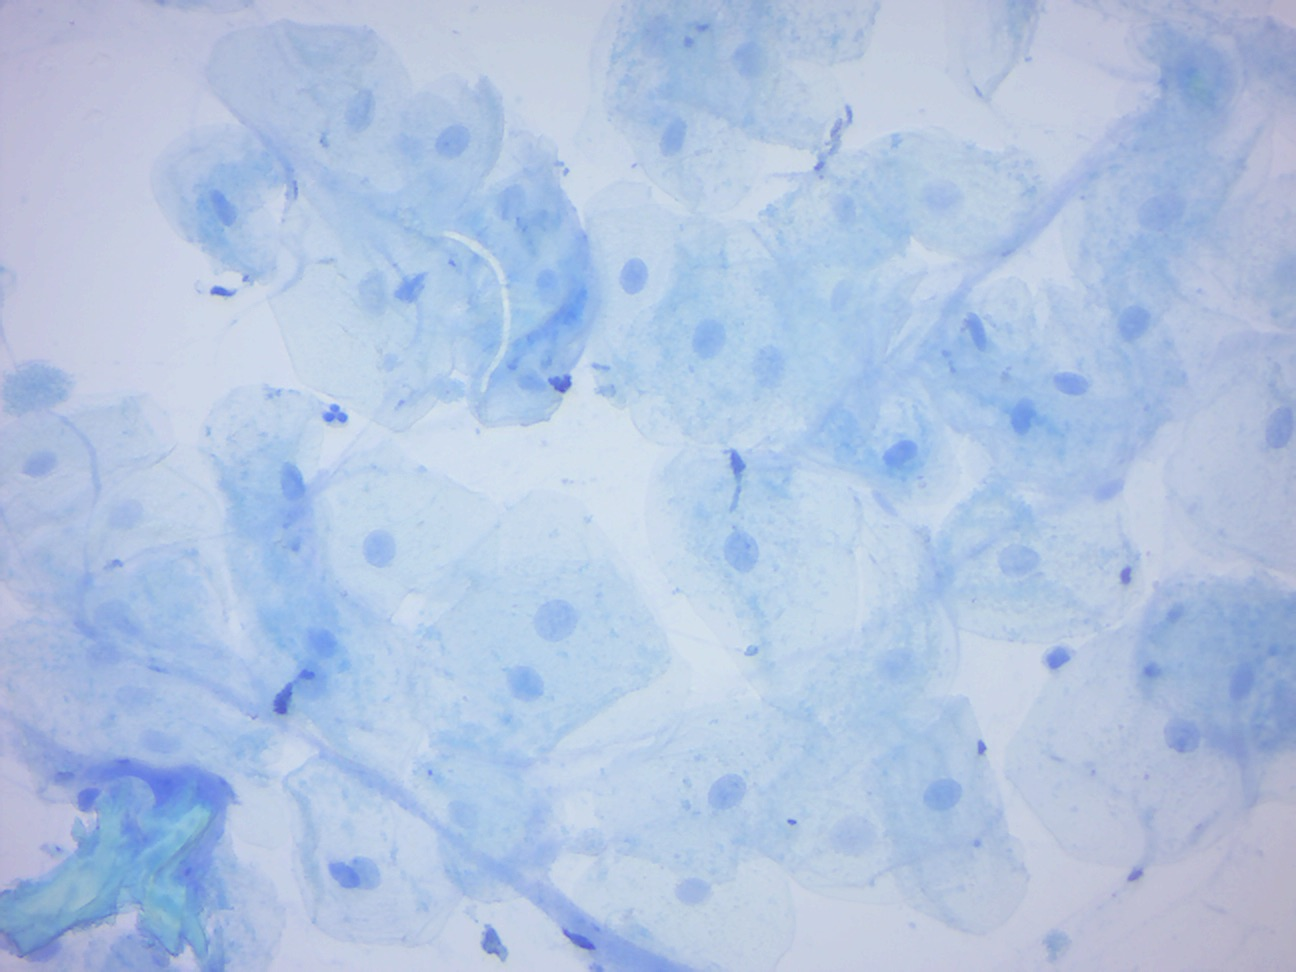
\includegraphics[width=0.7\linewidth]{./figures/cell_struc/cheek} 

}

\caption{Human cheek epidermal cells.}\label{fig:cheek}
\end{figure}

\section{Cleaning up}\label{cleaning-up-4}

Dispose of the toothpicks and the slide with the cheek cells in the
beakers containing (green looking) disinfectant liquid.

\section{Human blood cells}\label{human-blood-cells}

\href{https://en.wikipedia.org/wiki/Blood}{Blood} is a body fluid in
humans and other animals that delivers necessary substances such as
nutrients and oxygen to the cells and transports metabolic waste
products away from those same cells. In vertebrates, it is composed of
blood cells suspended in blood plasma. Plasma, which constitutes 55\% of
blood fluid, is mostly water (92\% by volume), and contains dissipated
proteins, glucose, mineral ions, hormones, carbon dioxide (plasma being
the main medium for excretory product transportation), and blood cells
themselves. Albumin is the main protein in plasma, and it functions to
regulate the colloidal osmotic pressure of blood. The blood cells are
mainly red blood cells (also called RBCs or erythrocytes), white blood
cells (also called WBCs or leukocytes) and platelets (also called
thrombocytes). The most abundant cells in vertebrate blood are red blood
cells. These contain hemoglobin, an iron-containing protein, which
facilitates oxygen transport by reversibly binding to this respiratory
gas and greatly increasing its solubility in blood. In contrast, carbon
dioxide is mostly transported extracellularly as bicarbonate ion
transported in plasma. Vertebrate blood is bright red when its
hemoglobin is oxygenated and dark red when it is deoxygenated. Some
animals, such as crustaceans and mollusks, use hemocyanin to carry
oxygen, instead of hemoglobin. Insects and some mollusks use a fluid
called hemolymph instead of blood, the difference being that hemolymph
is not contained in a closed circulatory system. In most insects, this
``blood'' does not contain oxygen-carrying molecules such as hemoglobin
because their bodies are small enough for their tracheal system to
suffice for supplying oxygen. Jawed vertebrates have an adaptive immune
system, based largely on white blood cells. White blood cells help to
resist infections and parasites. Platelets are important in the clotting
of blood. Blood is circulated around the body through blood vessels by
the pumping action of the heart. In animals with lungs, arterial blood
carries oxygen from inhaled air to the tissues of the body, and venous
blood carries carbon dioxide, a waste product of metabolism produced by
cells, from the tissues to the lungs to be exhaled.

\subsection{Experimental procedures}\label{experimental-procedures-12}

\begin{enumerate}
\def\labelenumi{\arabic{enumi}.}
\tightlist
\item
  Look at the prepared slide containing a human blood stain (Figure \ref{fig:blood}).
\item
  Can you distinguish multiple types of white blood cells?
\item
  Return the slide to the white slide box.
\end{enumerate}

\begin{figure}

{\centering 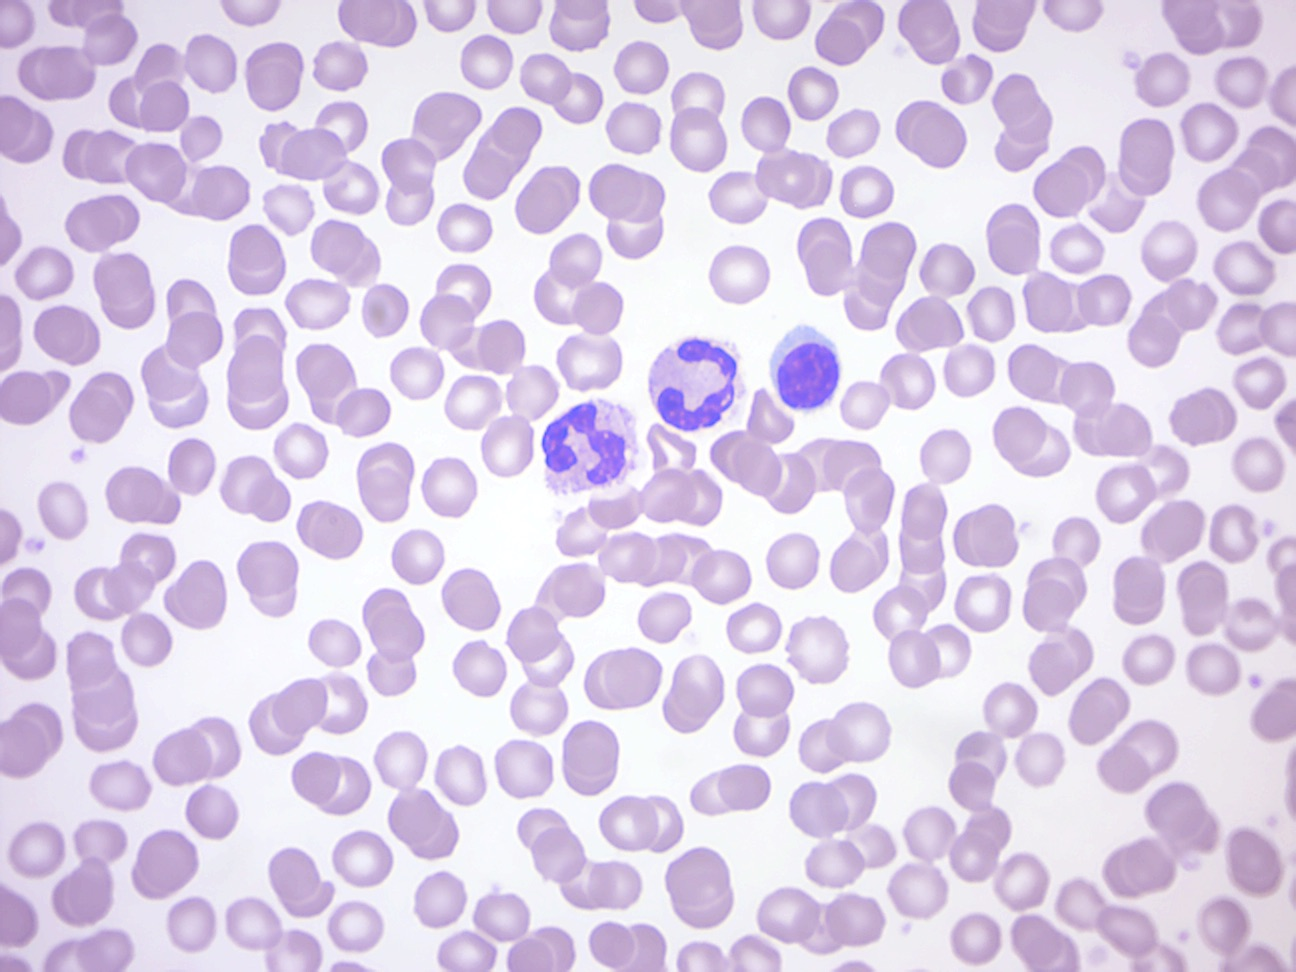
\includegraphics[width=0.7\linewidth]{./figures/cell_struc/blood} 

}

\caption{Human blood smear. Note red and two types of white blood cells.}\label{fig:blood}
\end{figure}

\section{Review Questions}\label{review-questions-2}

\begin{enumerate}
\def\labelenumi{\arabic{enumi}.}
\tightlist
\item
  What are the main structural features of eukaryotic cells?
\item
  What distinguishes animal cells from plant cells?
\item
  What are mitochondria?
\item
  What are chloroplasts?
\end{enumerate}
